\section{Distributed crawling(splitting by key range vs. hash of key)}\label{distcrawl}
This section presents strategies to distribute crawling activity across many nodes. Each participating
node is given the responsibility of downloading a slice of seed set. The main reason to distribute
crawling is to make it scalable.  
\\
\\
Mercator's\cite{mercator}(1999) host splitter component distributes load by hostname. Limitations of this way of distribution and alternatives are discussed below. Ubicrawler\cite{ubicrawler}(2004) achieved linear scalability, fault tolerance through consistent hashing\cite{consisthash}. Both designs mention some form of
load balancing however papers fall short of explanation on technicalities surrounding it.
\\
\\
When the goal is to distribute load evenly across finite number of nodes, say, 5 nodes should handle 5 times the throughput
of a single node. One way to split the load is to assign a range of request boundaries from minimum to
maximum to each node. Examples of load distribution based on range of keys can be hostnames, alphabets A-Z, etc. This works
as long as there exist calculated risk of every node getting a fair share of the load but in many cases,
load is unbalanced which causes one crawler node to compute more data than others causing skewed
workloads\cite{consisthash}. In extreme cases, only a specific boundary(e.g A-D) assigned to a node is taking all the load while other nodes responsible for handling boundary say X-Z, sits idle, such high disproportionate load becomes a hot spot\cite{consisthash} in distributed systems terminology.
\\
\\
To overcome problems encountered above with partitioning load by key range is to use hash function such that output of hash of a key is an integer which maps to a position somewhere on the line across the range of
numbers, shown in figure \ref{fig:requestboundary}. A hash function with low collision probability can
turn a skewed load into uniformly distributed load. Each physical machine/node $pn$ is hashed to a random integer between $0$ to $2^N-1$ where $N=16$ using a 16-bit hash function that serves range of hash values falling
within its request boundaries $RB_i$. Figure \ref{fig:requestboundary} shows $RB_i$ can be psuedorandomly or evenly spaced to fairly distribute load across $pn_i$.

\begin{figure}[h!]
  \centering
  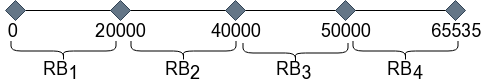
\includegraphics[width=10cm,height=4cm,keepaspectratio]{../media/crawler/requestboundaries.png}
  \caption{partitioning by hash of key}
  \label{fig:requestboundary}
\end{figure}

\pagebreak

\noindent
Certain attributes of a machine can be used as a input key to a hash function mapping to a integer on the
line figure \ref{fig:modnsplit}. From left to right, when hash of a absolute URL(e.g at 23000) used as a
key falls within a nodes range, task request is fulfilled by that node(at 40000). This way of distributing
the load evenly across machine is called consistent hashing\cite{consisthash}. Hashing reduces skewed
workloads and hot spots but they cannot be 100 percent eliminated.

\begin{figure}[h!]
  \centering
  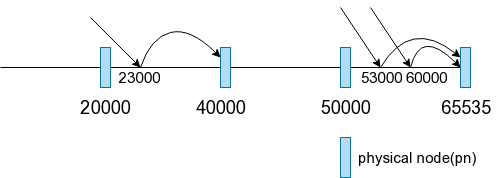
\includegraphics[width=10cm,height=4cm,keepaspectratio]{../media/crawler/modnsplit.png}
  \caption{Rebalancing physical nodes by mod N}
  \label{fig:modnsplit}
\end{figure}
\\
\\
\noindent
So far the assumption is parallel crawling will always be performed on a fixed number of $pn$ which is quite
unlikely. Overtime, a crawler's seed set may expand or shrink or altogether change its characteristics(see
figure \ref{fig:whrlplcrawlorder} requiring more CPU to cope up with or a node can crash for some
reason(e.g RAM overflow). All these changes mean moving messages between nodes. Once rebalancing is successfull, crawling load is distributed fairly among available nodes.
\begin{figure}[h!]
  \centering
  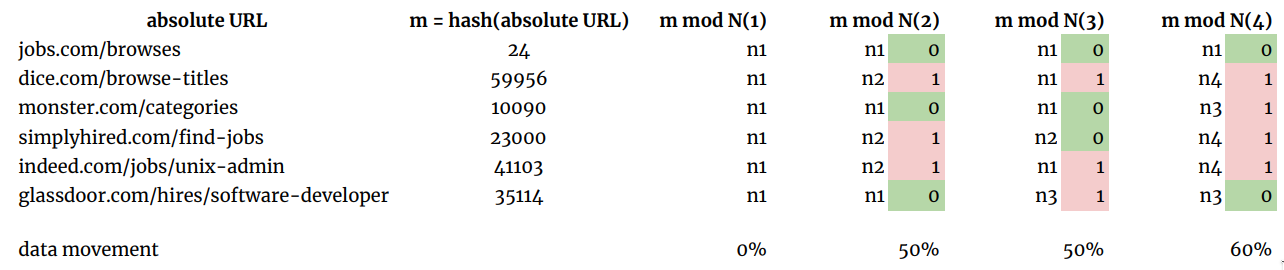
\includegraphics[width=16cm,height=8cm,keepaspectratio]{../media/crawler/modn_info.png}
  \caption{data movement when using modulo N}
  \label{fig:movemodn}
\end{figure}

\noindent
The easy strategy to rebalance request boundaries assigned to a node $pn_i$ is through $ph_i \equiv h(url)\mod{N}$, where $N$ is total number of available $pn_i$. For e.g, $h(url)\mod 5$ would direct service request
to any pnodes between 0 < $pn_i$ < 4. Figure \ref{fig:movemodn} shows a troubling trend with mod $N$ where
rebalancing of $N$ nodes causes half of service requests to redirect to another nodes. Every addition of
new node $pn_i$ has 50\% shift in service request, same happens in reverse. Note that the crawler program implemented for this thesis keeps state of URLs local to its message queue, therefore making rebalancing
with mod $N$ an expensive operation.

\pagebreak

\noindent
The problem is countered by iterating each $pn_i$ through few different hash functions and marking its positions on the line as shown in figure \ref{fig:vnodesplit1}. The values obtained are called virtual nodes(vnodes) $vn_i$ which are just essentially integers of different hash functions(in this case - $h_2$, $h_3$, $h_4$) and not virtualboxes running on real hardware. A rule of thumb is to have more number of $vn$ than there are $pn$ so
that several $vn$ are assigned to $pn$. For e.g a cluster of 3 pnodes has 12 vnodes where 4 vnodes are assigned to each pnode.

\begin{figure}[h!]
  \centering
  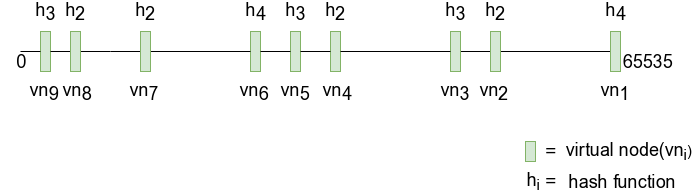
\includegraphics[width=12cm,height=5cm,keepaspectratio]{../media/crawler/vnodesplit1.png}
  \caption{virtual nodes to reduce shifts in data movements between nodes}
  \label{fig:vnodesplit1}
\end{figure}

\noindent
Once vnodes have positions on the line, pnodes are finally placed on the line with hash function quite different from that used for respective vnodes. Figure \ref{fig:vnodesplit2} shows 4 physical nodes, each running
an instance of rabbitMQ with crawler subsystems bound to them. This works differently from previous modulo N strategy. When a request comes in and its hash(44000) falls somewhere near to $vn_3$ who's hash value is 46000, it is consumed by pnode $pn_1$ at hash value 60000. Similarly, a hash value of 10 is near to $vn_9$ is served by $pn_4$. When a new pnode is added to the existing cluster, fewer vnodes from every pnode
$pn_i$ in the cluster get reassigned to newly added pnode and url is consumed by first pnode available on
the line, from left to right. The same thing happens in reverse when node is being removed from the cluster.
The criteria for load distribution can be, more powerful pnodes can take greater share of the load meaning
assigning more vnodes $vn$ for that particular pnodes $pn$.

\begin{figure}[h!]
  \centering
  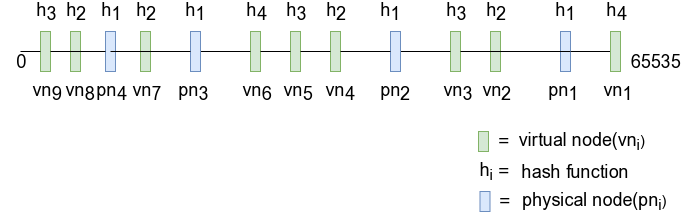
\includegraphics[width=12cm,height=5cm,keepaspectratio]{../media/crawler/vnodesplit2.png}
  \caption{Rebalancing physical nodes with virtual nodes}
  \label{fig:vnodesplit2}
\end{figure}

\pagebreak

\noindent
In order for crawler subsystems to know whether a current url is for itself or other pnodes in the cluster
(pnodes are actually crawler subsystems), even when pnodes are rebalanced and assignment of vnodes to
pnodes change, there exist a service discovery tool which keeps up-to-date information on ip address
and port number of pnodes in cluster and can thereby direct url request to the right pnode. The host
splitter makes the routing decision and learns about changes in the assignment of vnodes to pnodes. It
does so through zookeeper\cite{zookeeper} which is a coordination service for keeping metadata about
pnodes cluster.

\begin{figure}[h!]
  \centering
  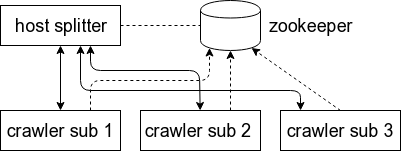
\includegraphics[width=8cm,height=5cm,keepaspectratio]{../media/crawler/zookeeper.png}
  \caption{zookeeper used to maintain up-to-date information on which vnodes are assigned to pnodes}
  \label{fig:zookeeper}
\end{figure}

\noindent
Each pnode $pn$ when available, registers itself with zookeeper. The zookeeper table in figure
\ref{fig:zookeeper_info} maintains mapping between vnodes $vn$ to pnodes $pn$. Host splitter subscribes
to zookeeper server. When a pnode is added or removed and vnodes are reassigned, zookeeper notifies host
splitter component.

\begin{figure}[h!]
  \centering
  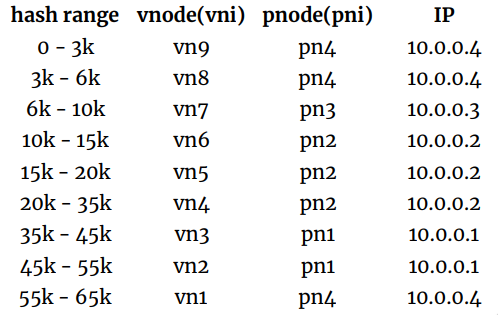
\includegraphics[width=10cm,height=8cm,keepaspectratio]{../media/crawler/zookeeper_info.png}
  \caption{zookeeper table}
  \label{fig:zookeeper_info}
\end{figure}

\pagebreak